\documentclass{standalone}
\usepackage[T1]{fontenc}
\usepackage[latin2]{inputenc}
\usepackage[english]{babel}
\usepackage{tikz}
\usepackage{times}
\usetikzlibrary{calc,through,backgrounds,positioning,fit}
\usetikzlibrary{shapes,arrows,shadows}
 
\begin{document}
 
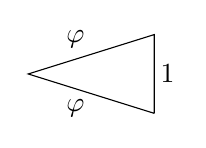
\begin{tikzpicture}[scale=1,inner sep=0.4mm]
\coordinate (p1) at (0,0);
\coordinate (p2) at (0,1);
\coordinate (p3) at (-1.6,0.5);

\coordinate (O) at (0,0.5);
\coordinate (q) at (-1,0.5);
\node at (O) [right=1pt] {$1$};
\node at (q) [above=8pt] {$\varphi$};
\node at (q) [below=8pt] {$\varphi$};

\draw (p1) -- (p2) -- (p3) -- (p1);
\end{tikzpicture}
 
\end{document}